\documentclass[12pt]{report}

%%%%%%%%%%%%%%%%%%%%%%%%%%
%%%%%% UNIT PREAMBLE %%%%% 
%%%%%%%%%%%%%%%%%%%%%%%%%%

% Basics 
\usepackage[utf8]{inputenc}
\usepackage[T1]{fontenc}
\usepackage{textcomp}
\usepackage[a4paper, left=1in, right=1in, top=1in, bottom=1in]{geometry}
\renewcommand\familydefault{\sfdefault}

\usepackage[Sonny]{fncychap}

\usepackage{amsmath,amsfonts,amsthm,amssymb,mathtools}
\usepackage[varbb]{newpxmath}
\usepackage{xfrac}
\usepackage[usenames,dvipsnames]{xcolor} % usenames, dvipsnames adds more colours
\usepackage{hhline}
\usepackage{comment}
\usepackage{tasks}
\usepackage{enumerate} 
\usepackage{enumitem} 
\usepackage{titlesec}
\usepackage[most]{tcolorbox}
\usepackage{lipsum}
\usepackage{tabularx}
\usepackage[labelfont=bf]{caption}
\usepackage{subfig}
\usepackage{pgfplots}
\usepackage{cancel} 
\usepackage{physics} 
\usepackage[bookmarks]{hyperref}
\usepackage{array}
\usepackage{float}
\usepackage{standalone}
\usepackage{graphicx}
\usepackage{forest}

% Tables 
\numberwithin{table}{section}

% Inkscape Figures
\usepackage{import}
\usepackage{xifthen}
\usepackage{pdfpages}
\usepackage{transparent}
\newcommand{\incfig}[2][1]{
    \def\svgwidth{#1\columnwidth}
    \import{../figures/}{#2.pdf_tex}
}

\pdfsuppresswarningpagegroup=1

% Chemistry
\usepackage{lewis} 
\usepackage{bohr}
\usepackage[version=4]{mhchem}

% Page setup
\hypersetup{hidelinks}
\pagenumbering{arabic}
\pagestyle{plain}
\setlength{\parindent}{0pt}

% Show subsubsections
\setcounter{tocdepth}{3}
\setcounter{secnumdepth}{3}

% Required for the Grid
\usetikzlibrary{calc}

% Section Font-Size
\titleformat{\subsubsection}
  {\normalfont\fontsize{12}{12}\bfseries}{\thesubsubsection}{1em}{}

\titleformat{\subsection}
  {\normalfont\fontsize{14}{14}\bfseries}{\thesubsection}{1em}{}

\titleformat{\section}
  {\normalfont\fontsize{16}{16}\bfseries}{\thesection}{1em}{}

% New page for each section 
\newcommand{\sectionbreak}{\clearpage}

% Section Spacing
\titlespacing{\section}{0em}{2.5em}{1em}
\titlespacing{\subsection}{0em}{2.5em}{1em}
\titlespacing{\subsubsection}{0em}{2.5em}{1em}

% TABLE COLUMN SEPARATION (USES ARRAY PACKAGE)
% \renewcommand{\arraystretch}{1.8} % changes vertical space for each cell 
% \setlength{\tabcolsep}{18pt} % changes horizontal space for each cell
% \setlength{\arrayrulewidth}{0.25mm}

% TCOLORBOX 
% \newtcolorbox[auto counter, number within=section]{definition}{colback=white,title=Example~\thetcbcounter,breakable,colframe=white,boxrule=0pt, enhanced, title style={left color=gray!60,right color=white,middle color=white},arc=0mm, titlerule=0pt, fonttitle=\bfseries\sffamily}

% Theorems 
\usepackage{thmtools}
\usepackage[framemethod=TikZ]{mdframed}

\declaretheoremstyle[
    headfont=\bfseries\sffamily\color{ProcessBlue!70!black}, bodyfont=\normalfont,
    headpunct= :,
    mdframed={
        linewidth=2pt,
        rightline=false, topline=false, bottomline=false,
        linecolor=ProcessBlue, backgroundcolor=ProcessBlue!5,
        innerbottommargin=10pt
    } ]{note}

\declaretheoremstyle[
    headfont=\bfseries\sffamily\color{NavyBlue!70!black}, 
    bodyfont=\normalfont,
    % headpunct=,
    mdframed={
        linewidth=2pt,
        rightline=false, topline=false, bottomline=false, linecolor=NavyBlue, innerbottommargin=10pt
    }
]{solution}

\declaretheoremstyle[
    headfont=\bfseries\sffamily\color{Gray!70!black}, bodyfont=\normalfont,
    % headpunct= ,
    postheadspace=\newline,
    mdframed={
        linewidth=2pt,
        rightline=false, topline=false, bottomline=false,
        linecolor=Gray, backgroundcolor=Gray!5,
        innerbottommargin=10pt
    } ]{remark}

\declaretheoremstyle[
    headfont=\bfseries\sffamily\color{Fuchsia!70!black}, bodyfont=\normalfont,
    % headpunct= ,
    mdframed={
        linewidth=2pt,
        rightline=false, topline=false, bottomline=false,
        linecolor=Fuchsia, backgroundcolor=Fuchsia!5,
        innerbottommargin=10pt
    }
]{example}

\declaretheoremstyle[
    headfont=\bfseries\sffamily\color{Fuchsia!70!black}, 
    bodyfont=\normalfont,
    % headpunct= ,
    mdframed={
        linewidth=2pt,
        rightline=false, topline=false, bottomline=false,
        linecolor=Fuchsia,
    }
]{examplesolution}

\declaretheoremstyle[
    headfont=\bfseries\sffamily\color{black!70!black}, 
    bodyfont=\normalfont,
    mdframed={
        linewidth=1pt,
        rightline=false, topline=false, bottomline=false,
        linecolor=black,
    }
]{definition}

\declaretheorem[style=solution, name=Solution, numbered=no]{solution}

\declaretheorem[style=solution, name=Derivation, numbered=no]{derivation}

\declaretheorem[style=definition, name=Definition, numberwithin=chapter]{definition}

\declaretheorem[style=note, name=Note, numbered=no]{noteswap}
\newenvironment{note}[1]{\vspace{0.5em}\begin{noteswap}[#1]}{\end{noteswap}\vspace{0.5em}}

\declaretheorem[style=remark, name=Remark, numbered=no]{remarkswap}
\newenvironment{remark}{\vspace{0.5em}\begin{remarkswap}}{\end{remarkswap}\vspace{0.5em}}

\declaretheorem[style=example, name=Example, numbered=no]{exampleswap}
% \newenvironment{example}{\vspace{0.5em}\begin{exampleswap}}{\end{exampleswap}}

\declaretheorem[style=examplesolution, name=Solution, numbered=no]{examplesolutionswap}
\newenvironment{examplesolution}{\vspace{-2em}\begin{examplesolutionswap}}{\end{examplesolutionswap}}

% Enumerate environments 
\newenvironment{2qu}
{
\begin{enumerate}[label=(\alph*)]
}
{\end{enumerate}}

\newenvironment{3qu}
{
\begin{enumerate}[label=(\roman*)]
}
{\end{enumerate}}

% Normal Environments 
\newenvironment{list0.5}
{
\begin{enumerate}
\setlength\itemsep{0.5em}
}
{\end{enumerate}}

% \titleformat{\section}{\vbox{\rule{\linewidth}{0.8pt}}\bigskip\LARGE\bfseries}{\thesection}{1em}{}

\titleformat{\section}
  {\normalfont\Large\bfseries}{\thesection}{1em}{}[{\titlerule[0.8pt]}] % horizontal line below

% thmtools Environments
\newenvironment{problems}
{
    \subsection{Problems}
    \begin{enumerate}
    \setlength\itemsep{1em}
}
{\end{enumerate}}

\newenvironment{+problems}
{
    \subsubsection{Problems}
    \begin{enumerate}
    \setlength\itemsep{1em}
}
{\end{enumerate}}

\newenvironment{example}[1]
{
    \begin{exampleswap}
        #1
    \end{exampleswap}
    \begin{examplesolution}
}
{
\end{examplesolution}}

\newenvironment{2example}[1]
{
    \begin{exampleswap}[#1]
}
{
\end{exampleswap}}

% Managing Figures
\captionsetup{width=0.8\textwidth}
\renewcommand{\thefigure}{\arabic{chapter}.\arabic{figure}}

% TABLE
% \begin{table}[h!] % delete [h!] if there are bugs

%     %%% TABLE CONFIG %%% 
%     \renewcommand{\arraystretch}{1.5} % changes vertical space for each cell 
%     \setlength{\tabcolsep}{10pt} % changes horizontal space for each cell
%     \setlength{\arrayrulewidth}{0.25mm}

%     \begin{center}
%          title of the table \
%         \vspace{0.5em}
%         \begin{tabular}{|c|c|} % use r, l, c for right, left, center. use m{3cm} for middle width of 3cm, use  b{3cm} for bottom width of 3cm, and use p{3cm} for a top width of 3cm.  
%         \hline
%          &  \ % two columns corresponding to two c's
%         \hline
%          &  \ % second row
%         \hline
%         \end{tabular}
%     \end{center}
%     \caption{}
% \end{table}

% Symbols 
\newcommand{\z}{\mathbb{Z}}

\renewcommand{\l}{\ell}

% Formatting 
\newcommand{\invis}{\vphantom{Invisible Text}}
\newcommand{\divider}{\par\noindent\rule{\textwidth}{0.5pt}\vspace{0.4em}}

% Chemistry
% \newcommand{\2ch}[2]{\ce{#1}_{(#2)}}
% \newcommand{\io}[2]{\text{#1}^{#2}} 
% \newcommand{\2io}[3]{\text{#1}^{#2}_{#3}}


\begin{document}

\newpage
\section{Respiratory System}
\marginpar{Monday \text{April 3 2023}}
\begin{definition}[Respiratory System]
    Responsible for providing oxygen to the body and removing carbon dioxide from the body. See Figure \ref{fig:respiratory-system} (a).
\end{definition}

\begin{figure}[!htb] 
    \centering
    \subfloat[\centering The lungs are protected by ribs.]{{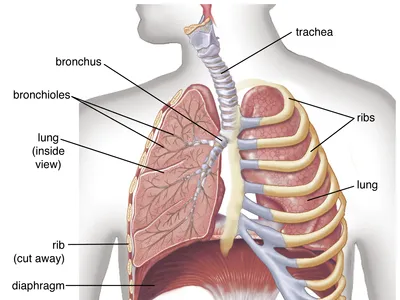
\includegraphics[width=0.45\textwidth]{../figures/respiratory system.png}}}  
    \qquad
    \subfloat[\centering The alveoli are in the lungs (search chatGPT for what this does).]{{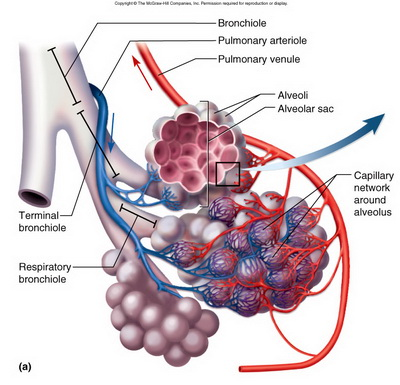
\includegraphics[width=0.45\textwidth]{../figures/alveoli.jpg}}}  
    % TODO
    \caption{The respiratory system.}
    \label{fig:respiratory-system}
\end{figure}

\subsection{Nose/Mouth}
\begin{definition}[Nose/Mouth]
    Where air enters and passes through the pharynx (throat). 
    \begin{itemize}
        \item{Mucous and hairs trap small particulates.}
        \item{Capillaries in the nose warm the air.}
    \end{itemize}
\end{definition}

\subsection{Larynx}
\begin{definition}[Larynx]
    For sound production and also functions to protect the lower airways by closing or coughing.
\end{definition}

\subsection{Trachea}
\begin{definition}[Trachea]
    The windpipe that is surrounded by cartilage rings to prevent collapse. The very top is the voice box, and it branches off into the bronchi, which eventually branches off into the lungs. See Figure \ref{fig:trachea}.
\end{definition}

\begin{figure}[H]
\centering
    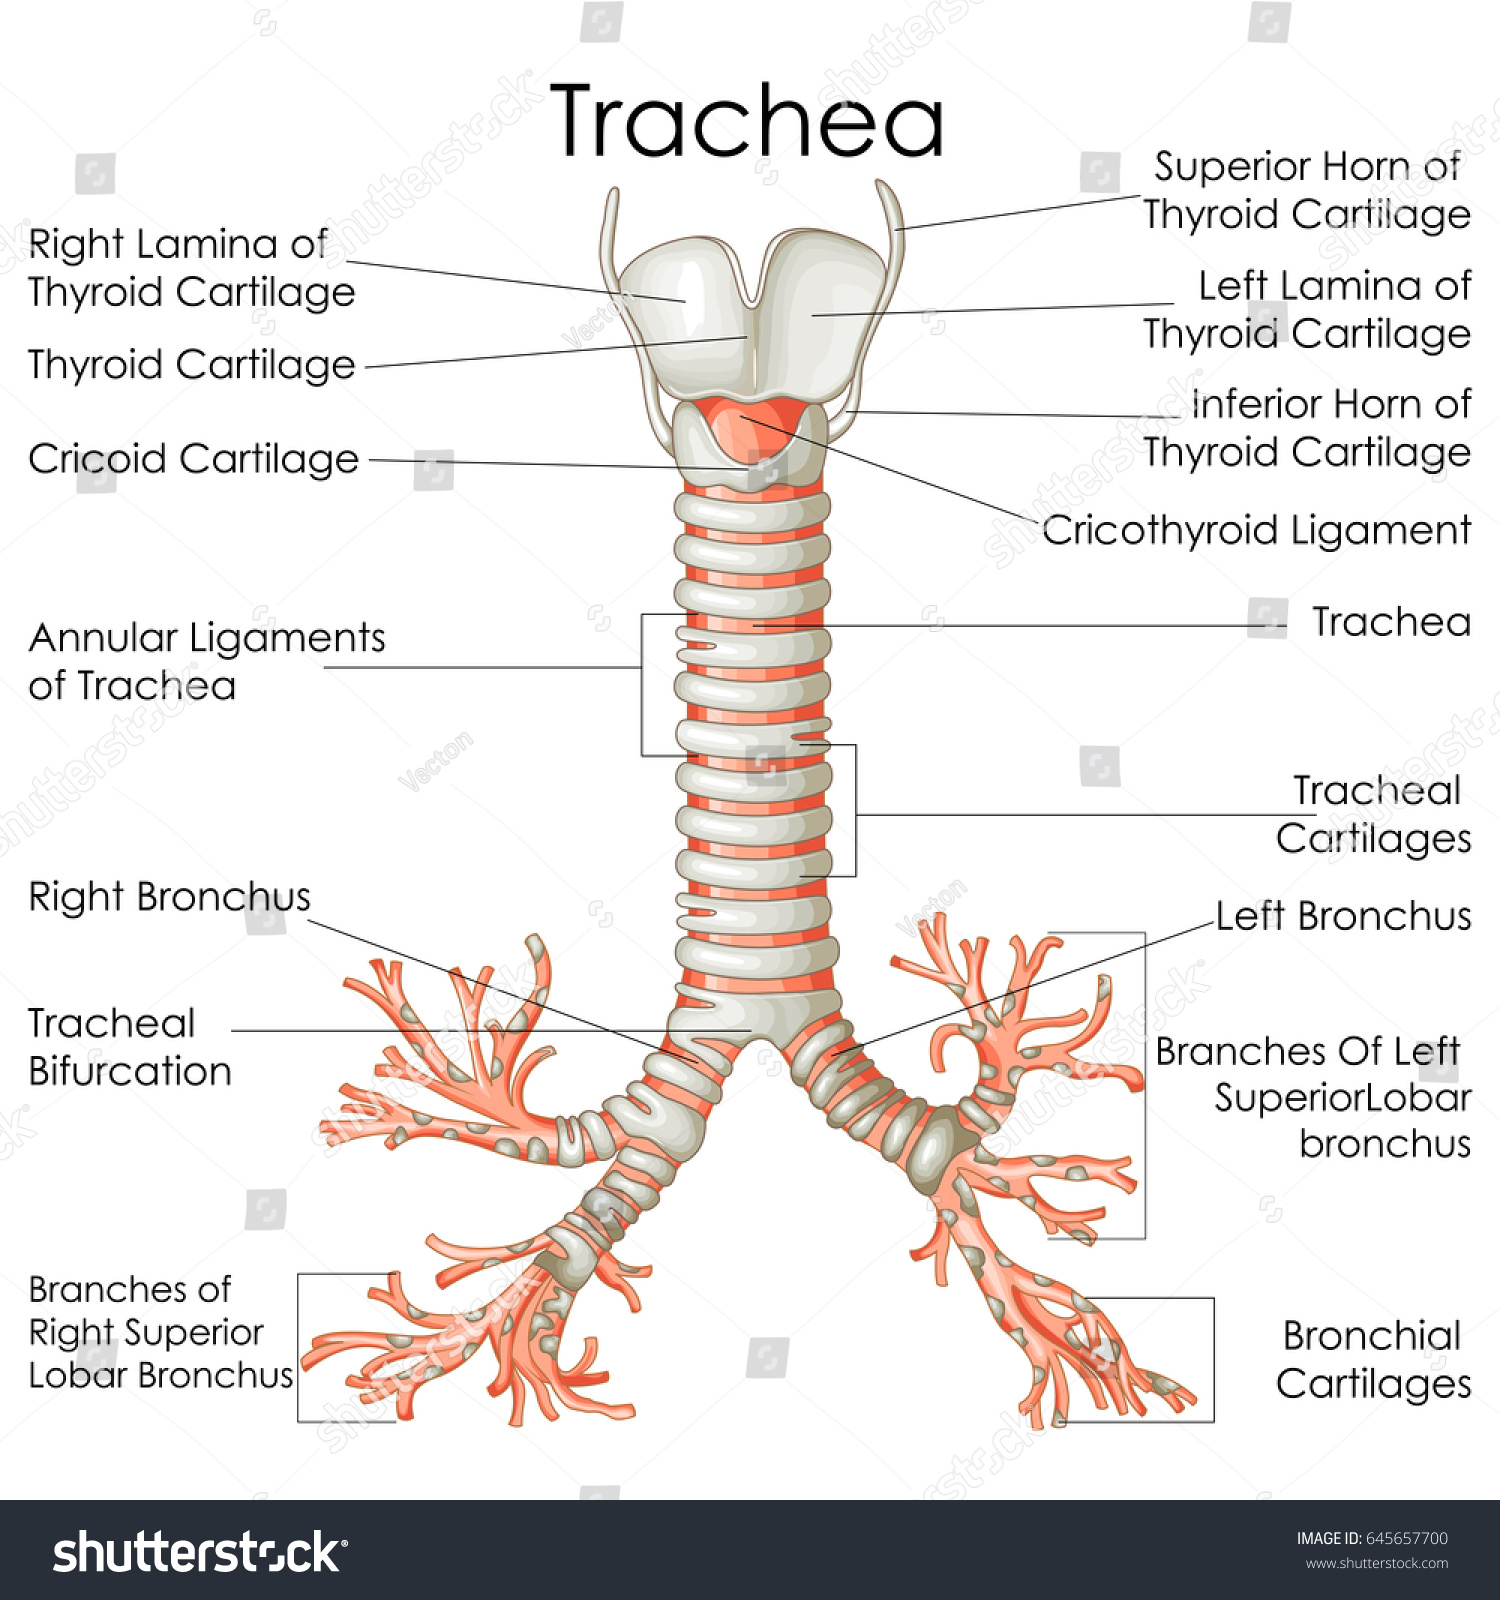
\includegraphics[width=0.5\textwidth]{../figures/trachea.jpg}
    \caption{The trachea branches off into the lungs.}
    \label{fig:trachea}
\end{figure}

\subsection{Bronchi}
\begin{definition}[Bronchi]
    Where the trachea splits into the left and right bronchus.
    \begin{itemize}
        \item{Contains goblet cells in the epithelial lining to produce mucus.}
        \item{Lined with cilia (hair-like projections) to sweep materials out of the lower airway.}
    \end{itemize}
\end{definition}

\subsection{Bronchioles}
\begin{definition}[Bronchioles]
    Where the bronhi splits into smaller tubes.
\end{definition}

\divider 

\subsection{In the Lungs: Alveoli}
\begin{definition}[In the Lungs: Alveoli]
    Tiny, capillary-bound sacs where gas exchange occurs between air and blood. See Figure \ref{fig:respiratory-system} (b) and Figure \ref{fig:alveoli}.
    \begin{itemize}
        \item{Membranes are thin to maximize diffusion.}
    \end{itemize}
    A better way to put it, from Figure \ref{fig:alveoli}, you can see that the alveoli and capillary are actually separated. How it works is that oxygen from the $ \text{bronchioles}\to \text{alveoli}$ gets diffused across and turns into carbon dioxide. Similarly, oxygen from the capillary itself gets diffused across and becomes deoxygenated as well.
\end{definition}

\begin{figure}[H]
\centering
    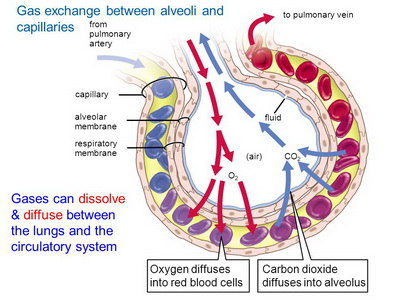
\includegraphics[width=0.7 \textwidth]{../figures/alveoli2.jpg}
    \caption{The oxygen diffuses (from blue to purple to red) and carbon dioxide is diffused out.}
    \label{fig:alveoli}
\end{figure}

\subsection{Pulmonary Arties and Capillaries}
\begin{definition}[Pulmonary Arties and Capillaries]
    Provides a large supply of deoxygenated blood to alveoli.
\end{definition}

\subsection{Pulmonary Veins}
\begin{definition}[Pulmonary Veins]
    Brings oxygenated blood back to the heart to be distributed to the rest of the blood.
\end{definition}

\subsection{Checkpoint: Pulmonary Fibrosis}
Pulmonary Fibrosis is when the tissue around the alveoli thickens and scars. How will this affet gas exchange?\\ 

\textbf{Solution:} The scar tissue will make gas exchange less efficient; this will result in a slowing down of the gas exchange, and will mean that the body's cells won't get rid of waste or get a delivery of oxygen as quickly as normal.

\subsection{Breathing}
\begin{definition}[Breathing]
    The process of breathing is caused by pressure differences between the atmosphere and the inside of the lungs.\\ 

    Air moves from an area of high pressure to low pressure.
    \begin{itemize}
        \item{Pressure can be changed by changing volume.}
            \begin{itemize}
                \item{Volume increases, pressure decreases. For example, imagine a balloon.}
                \item{Volume decreases, pressure increases.}
            \end{itemize}
    \end{itemize}
    The equation is $V\propto \frac{1}{p}.$
\end{definition}

\subsection{Lung Volume}
\begin{definition}[Lung Volume]
    Lung volume can be changed by: 
    \begin{itemize}
        \item{Contraction or relaxion of muscles in the rib cage.}
        \item{Contraction or relaxion of the \textbf{diaphragm,} which is a dome-shaped muscle underneath the lungs.}
    \end{itemize}
    In other words, when you inhale, the diaphragm compresses, and your lungs expand. When you exhale, this is when the diaphragm ``relaxes'', and is when it gets back into its normal shape, casugint he lungs to get smaller and greater air pressure within the lungs.
\end{definition}

\marginpar{Tuesday \text{April 4 2023}}

\subsection{Inhalation}
\begin{definition}[Inhalation]
    \invis
    \begin{itemize}
        \item{Rib cage expands.}
        \item{Diaphragm contracts and flattens.}
        \item{Lung volume increases.}
        \item{Lung pressure decreases.}
    \end{itemize}
    \textbf{Air moves in.}
\end{definition}

\subsection{Exhalation}
\begin{definition}[Exhalation]
    \invis
    \begin{itemize}
        \item{Rib cage contracts.}
        \item{Diaphragm relaxes and arches.}
        \item{Lung volume decreases.}
        \item{Lung pressure increases.}
    \end{itemize}
    \textbf{Air moves out.}
\end{definition}

\subsection{Respiratory System in Fish}
\begin{definition}[Respiratory System in Fish]
    \invis
    \begin{itemize}
        \item{Gas exchange occurs in the \textbf{gills}, which is a highly folded structure to maximize surface area.}
        \item{Undergoes countercurrnt exchang to maximize oxygen uptake from water.}
        \item{Gills are surrounded by capillaries to bring blood close to the water.}
    \end{itemize}
\end{definition}

\subsection{Diseases of the Respiratory System}
\begin{table}[h!]
    \renewcommand{\arraystretch}{1.5}
    \setlength{\tabcolsep}{10pt}
    \setlength{\arrayrulewidth}{0.25mm}

    \begin{center}
        \vspace{0.5em}
        \begin{tabular}{|l|p{0.5 \textwidth}|}
        \hline
         & Tuberculosis \\ 
        \hline
        Description & Bacterial infection that mainly affects the lungs but can spread to other parts of the body. \\
        \hline
        Symptoms & Coughing for 3 or more weeks. Coughing up blood or mucous. Chest pain.\\ 
        \hline 
        Causes & \textit{Mycobacterium tuberculosis} is a bacterium that attacks the lungs.\\ 
        \hline 
        Treatment & Antibiotics\\ 
        \hline
        \end{tabular}
    \end{center}
    \caption{Tuberculosis}
\end{table}

\begin{table}[h!]
    \renewcommand{\arraystretch}{1.5}
    \setlength{\tabcolsep}{10pt}
    \setlength{\arrayrulewidth}{0.25mm}

    \begin{center}
        \vspace{0.5em}
        \begin{tabular}{|l|p{0.5 \textwidth}|}
        \hline
         & Pneumonia \\ 
        \hline
        Description & Inflammation of the alveoli; alveoli may be filled with fluid or pus. \\
        \hline
        Symptoms & Coughing, chest pain, fever.\\ 
        \hline 
        Causes & Bacterial, viral, o rfungal infection.\\ 
        \hline 
        Treatment & \\
        \hline
        \end{tabular}
    \end{center}
    \caption{Pneumonia}
\end{table}

\begin{table}[h!]
    \renewcommand{\arraystretch}{1.5}
    \setlength{\tabcolsep}{10pt}
    \setlength{\arrayrulewidth}{0.25mm}

    \begin{center}
        \vspace{0.5em}
        \begin{tabular}{|l|p{0.5 \textwidth}|}
        \hline
         & COVID-19 \\ 
        \hline
        Description & A respiratory illness caused by the coronavirus called SARS-CoV-2 \\
        \hline
        Symptoms & Fever, cough, difficult breathing.\\ 
        \hline 
        Causes & SARS-CoV-2 virus\\ 
        \hline 
        Treatment & \\ 
        \hline
        \end{tabular}
    \end{center}
    \caption{COVID-19}
\end{table}

\begin{note}{Pneumonia on lungs}
When someone is experiencing pneumonia as a result of COVID-19, the lungs in an x-ray wion't be dark.
\end{note}

\section{Musculoskeletal System}
\begin{definition}[Musculoskeletal System]
    The organ system that conssits of muscles and bones. Function: 
    \begin{itemize}
        \item{Supports the body.}
        \item{Protects delicate organs.}
        \item{Movement.}
    \end{itemize}
\end{definition}

\subsection{Bone}
\begin{definition}[Bone]
    A hard and dense tissue that consists of bone cells within a matrix of minerals like calcium and phosphorus. Canals inside in the bones contain nerves and blood vessels.
\end{definition}

\subsection{Ligament}
\begin{definition}[Ligament]
    A tough, elastic tissue that holds bones together at the joints. 
\end{definition}

\subsection{Cartilage}
\begin{definition}[Cartilage]
    A dense tissue that provides storng, low-friction support for bones.    
\end{definition}

\subsection{Tendon}
\begin{definition}[Tendon]
    A connective tissue that connects muscles to bones.
\end{definition}

\subsection{Muscle Types}
\begin{definition}[Muscle Types]
    Muscle conssits of long bundles of muscle fibres that contain protein like actin and myosin for contraction. Types: 
    \begin{itemize}
        \item{ \textbf{Skeletal Muscle} (voluntary).}
        \item{ \textbf{Smooth Muscle} (involuntary).}
        \item{ \textbf{Cardiac Muscle} (heart).}
    \end{itemize}
\end{definition}

\subsection{Musculoskeletal System in Invertebrates}
\begin{definition}[Musculoskeletal System in Invertebrates]
    All vertebrates have Musculoskeletal systems. Intvertebrates have other adaptations for structure and support: 
    \begin{itemize}
        \item{Jellyfish rely on water to provide structural support.}
        \item{Worms have muscles that work against bodyfluids.}
        \item{Insects and arthropods have exoskeleton.}
    \end{itemize}
\end{definition}

\subsection{Diseases of the Musculoskeletal System}
\begin{table}[h!]
    \renewcommand{\arraystretch}{1.5}
    \setlength{\tabcolsep}{10pt}
    \setlength{\arrayrulewidth}{0.25mm}

    \begin{center}
        \vspace{0.5em}
        \begin{tabular}{|l|p{0.5 \textwidth}|}
        \hline
         & Osteoporosis \\ 
        \hline
        Description & A diseases thatcauses bones to become weak and brittle because the creation of new bones does not keep up with loss of old bone. \\
        \hline
        Symptoms & Back pain, loss of height over time, stooped poosture.\\ 
        \hline 
        Causes & Age, hormones, poor diet.\\ 
        \hline 
        Treatment & Drugs like bisphosphonates, hormon-related therapy.\\ 
        \hline
        \end{tabular}
    \end{center}
    \caption{Osteoporosis}
\end{table}

\marginpar{Wednesday \par{April 5 2023}}
\section{Nervous System}
\begin{definition}[Nervous System]
    The organ system that senses the environment and coordinates appropriate reponses. 
    \begin{itemize}
        \item{ \textbf{Central nervous system (CNS)} consists of the brain and spinal cord. The brain is protected by the skull and the spinal cord is protected by the spine.}
        \item{ \textbf{Peripheral nervous system (PNS)} consists of the nerves in the rest of the body.}
    \end{itemize}
    See Figure \ref{fig:nervous-system}.
\end{definition}

\begin{figure}[H]
\centering
    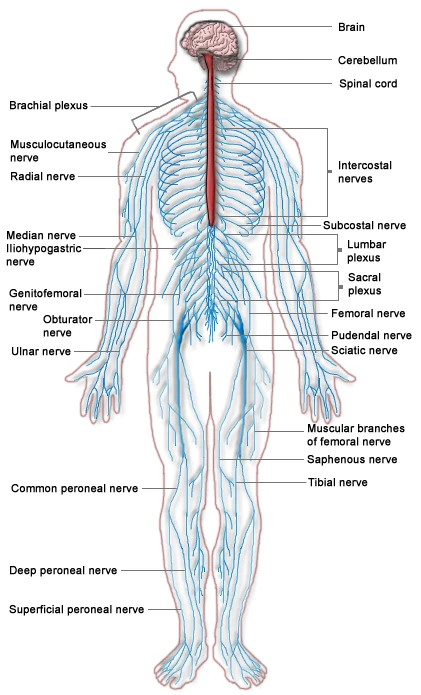
\includegraphics[width= 0.5\textwidth]{../figures/nervous system.png}
    \caption{The nervous system.}
    \label{fig:nervous-system}
\end{figure}

\subsection{Central Nervous System}
\begin{definition}[Central Nervous System]
    The brain consists of over billions of neurons and synapses. 
    \begin{itemize}
        \item{Protected by the skull and cerebrospinal fluid.}
    \end{itemize}
\end{definition}

\begin{figure}[H]
\centering
    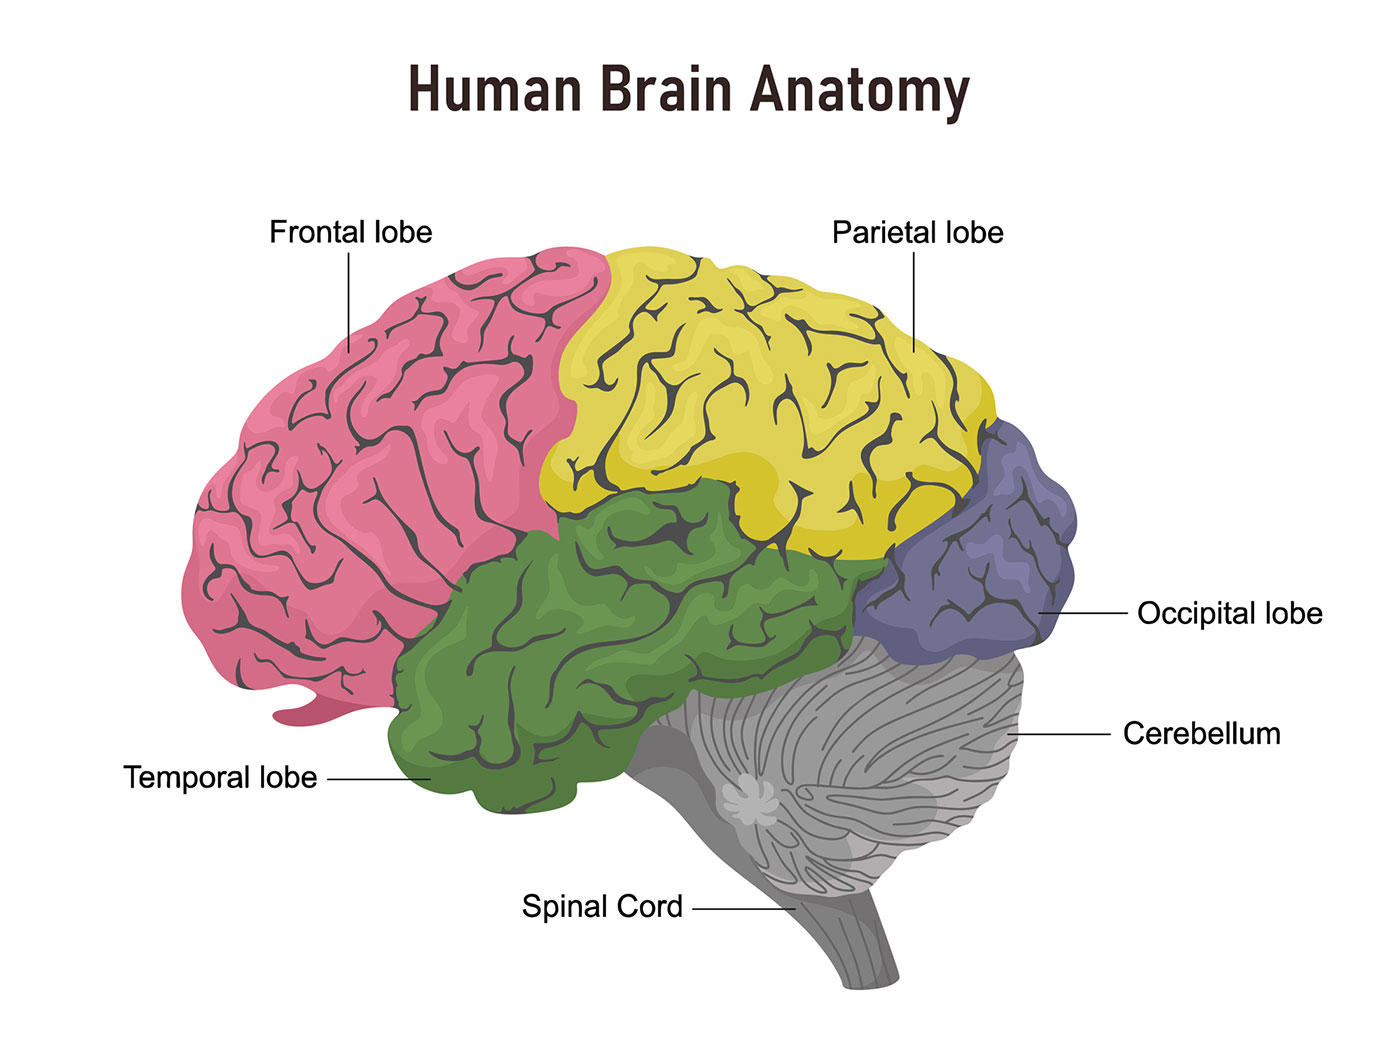
\includegraphics[width=0.5 \textwidth]{../figures/brain.jpg}
    \caption{The brain is like tofuu. In the tofuu, there is some water that protects the tofuu. The cerebralspinal fluid acts like that water in the tofuu.}
    \label{fig:brain}
\end{figure}

\subsection{Spinal Cord}
\begin{definition}[Spinal Cord]
    A long, fragile tube ofn erves that carries signals between the brain and body. 
    \begin{itemize}
        \item{The spinal cord is protected by the spine.}
    \end{itemize}
\end{definition}

\begin{figure}[H]
\centering
    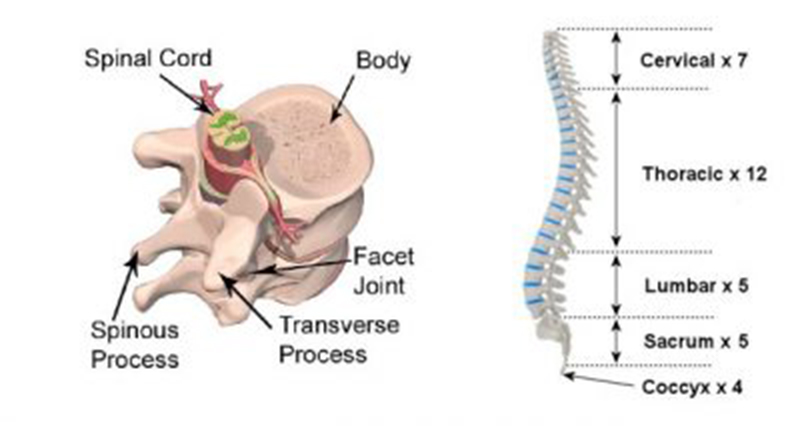
\includegraphics[width=0.5 \textwidth]{../figures/spinal cord.jpg}
    \caption{The spina cord (on the left) and the spine (on the right).}
    \label{fig:spinal-cord}
\end{figure}

\subsection{Peripheral Nervous System}
\begin{definition}[Peripheral Nervous System]
    \invis
    \begin{itemize}
        \item{The \textbf{neuron} is a nervec cell that sends electrical impulses to the target cell.}
        \item{\textbf{Myelin sheath} is a fatty material that covers the axon; acts as insulation to allow for electricla impulses to travel quickly tand from to the wrong neuron.}
    \end{itemize}
\end{definition}

\subsection{Nerve}
\begin{definition}[Nerve]
    A bundle of neurons. Types of nerves: 
    \begin{itemize}
        \item{Nerves for voluntary muscles.}
        \item{Nerve for involuntary functions.}
        \item{Nerves for sensory organs.}
    \end{itemize}
\end{definition}

\subsection{Sensory Receptors}
\begin{definition}[Sensory Receptors]
    Receive information from the external environment to be processed by the brain. 
    \begin{itemize}
        \item{Receptors sense sight, touch, temperature, taste, smell, sound, pressure, pain, balance, stretch, position.}
    \end{itemize}
\end{definition}

\subsection{Reflexes}
\begin{definition}[Reflexes]
    Actions that do not require the brain and occur without conscious thought through a reflex arc in the spinal cord.
    \begin{itemize}
        \item{Reflexes are intended to prevent injury and protect us from danger.}
        \item{Types:}
            \begin{itemize}
                \item{Deep-tendon reflex.}
                \item{Withdrawal reflex.}
                \item{Startle reflex.}
                \item{Blink reflex.}
                \item{Gag reflex.}
            \end{itemize}
        \end{itemize}
        See Figure \ref{fig:reflexes}.
\end{definition}

\begin{figure}[H]
\centering
    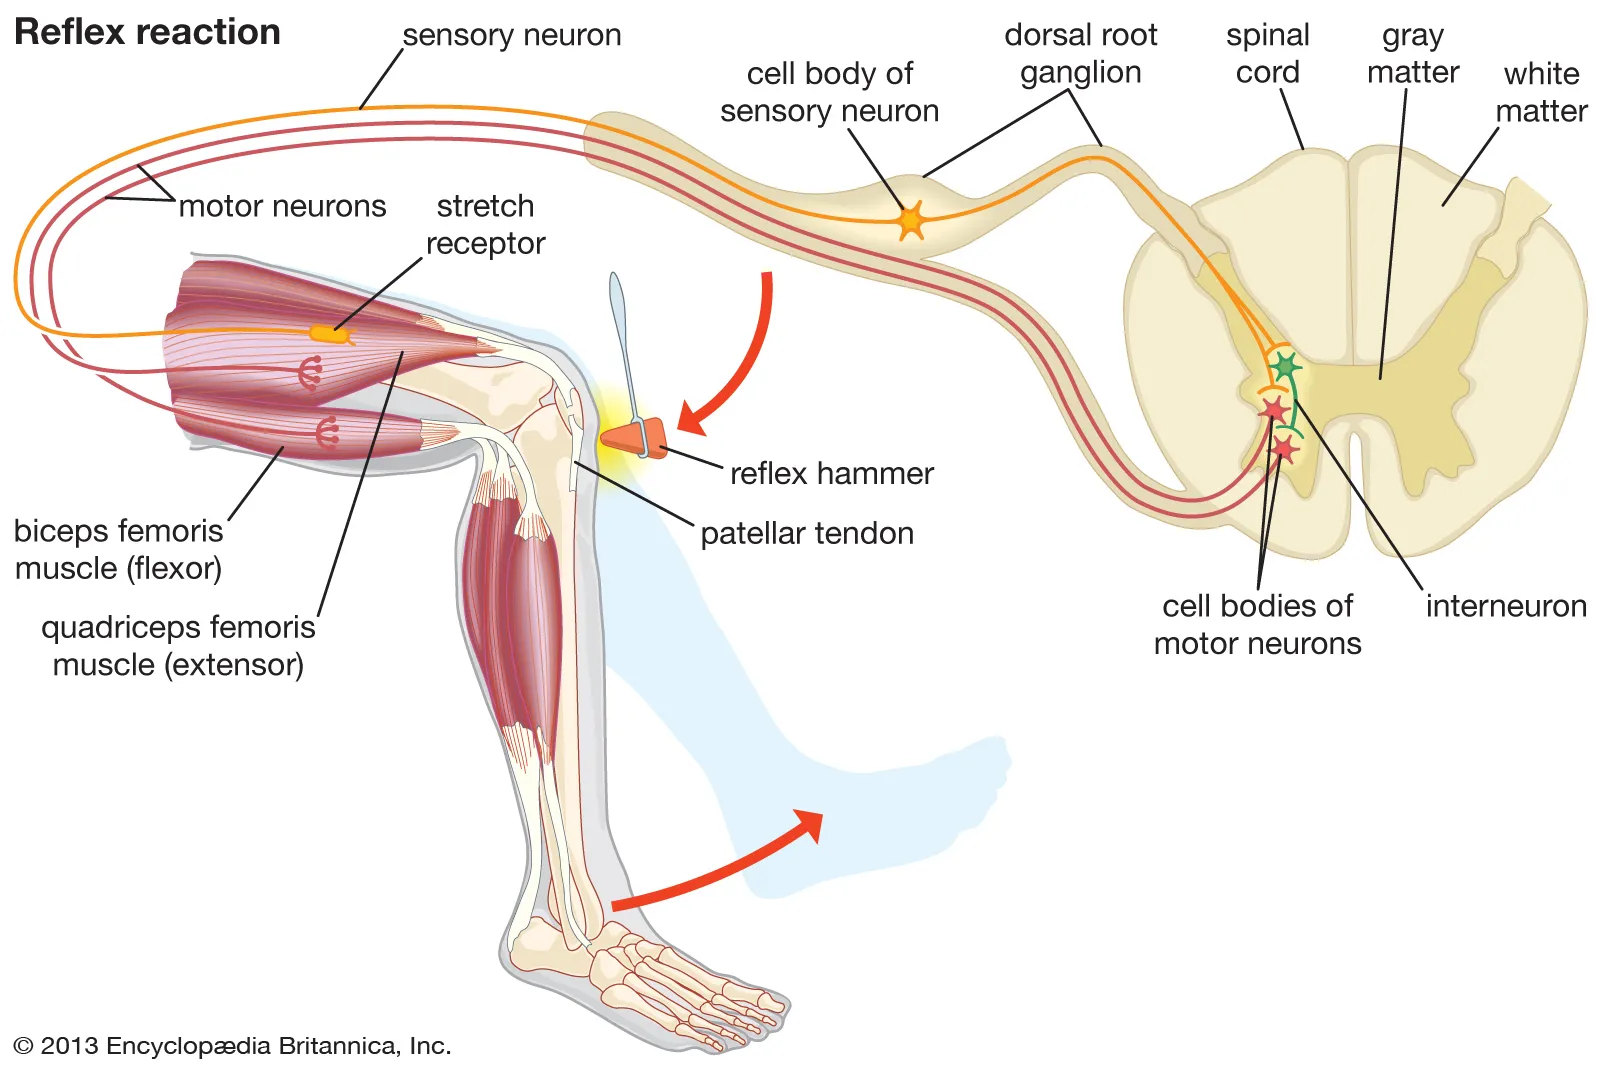
\includegraphics[width=0.5\textwidth]{../figures/reflexes.png}
    \caption{The doctor will hit your knee, and usually you will kick. If you do not kick, something is wrong.}
    \label{fig:reflexes}
\end{figure}

\subsection{Diseases of the Nervous System}
\begin{table}[h!]
    \renewcommand{\arraystretch}{1.5}

    \begin{center}
        \vspace{0.5em}
        \begin{tabular}{|p{0.3 \textwidth}|p{0.7 \textwidth}|}
        \hline
         & Multiple Scelrosis \\ 
        \hline
        Description & Myelin sheaths in the central nervous system deteriorates leading to nerve damage. \\
        \hline
        Symptoms & Numbness or weakness in one or more limbs. Electric-shock sensations. Tremor, lack of coordinate.\\ 
        \hline 
        Causes & Autoimmune diases; the body is attacking its own mecahnism.\\ 
        \hline 
        Treatment & No cure. Drugs to reduce nerve inflammation. Drugs to modify progression.\\ 
        \hline
        \end{tabular}
    \end{center}
    \caption{Multiple Scelrosis}
\end{table}

\begin{figure}[H]
\centering
    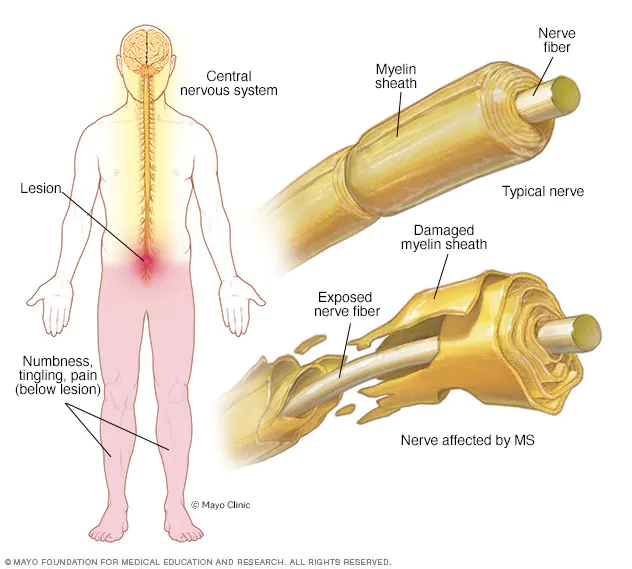
\includegraphics[width=0.5 \textwidth]{../figures/multiple scelrosis.png}
    \caption{Multiple scelrosis; damaged myelin sheath.}
    \label{fig:multiple-scelrosis}
\end{figure}

\begin{table}[h!]
    \renewcommand{\arraystretch}{1.5}
    \setlength{\tabcolsep}{10pt}
    \setlength{\arrayrulewidth}{0.25mm}

    \begin{center}
        \vspace{0.5em}
        \begin{tabular}{|l|l|}
        \hline
         & Concussion \\ 
        \hline
         Description & Brain injury that affects brain function. \\
        \hline
         Symptoms & Headache, ringing in the ears, nausea and vomiting, amnesia.\\ 
         \hline 
         Causes & Trauma to the head from a fall or sports. Violent shaking of upper body.\\ 
         \hline 
         Treatment & Physical and mental rest. Pain relief medication.\\ 
         \hline
        \end{tabular}
    \end{center}
    \caption{Concussion}
\end{table}

\marginpar{Thursday \par{April 6 2023}}
\subsection{Organ Transplant}
\begin{definition}[Organ Transplant]
    Sugery where the organ or tissue of the donor is given to the recipient to replace a damaged organ or tissue. Organ transplants have been performed since the early 1800s when blood transfusions were explored.
\end{definition}

\subsection{Types of Organ Donors}
\begin{definition}[Types of Organ Donors]
    \invis 
    \begin{itemize}
        \item{ \textbf{Invis donor organs} are organs that come from a living person - usually a family member with similar genetic traits to avoid rejection by the immune system. Ex: kidney, lobe of lungs, part of the liver.}
        \item{ \textbf{Deceased donor organs} are organs that come from a dead person.}
        \item{ \textbf{Xenotransplantation} is the transplanting of body parts from one species of another. Ex: heart valves from pigs.}
    \end{itemize}
\end{definition}

\subsection{Organ Trafficking}
\begin{definition}[Organ Trafficking]
    The practiec of stealing or buying organs through exploitation, coercion, or fraud. Low supply of organs but a high demand for organ transplants lead to a black market. Most common trafficking organs are kidneys.
\end{definition}

\end{document}
